\section{OMPD}
\label{sec:ompd-overview}
\label{sec:third-party-tool-callback-interface}

The OMPD interface is designed to allow a \emph{third-party tool}
such as a debugger to inspect the OpenMP state of a live program
or core file in an implementation agnostic manner.
That is, a tool that uses OMPD should work with any conforming
OpenMP implementation.
The model for OMPD is that an OpenMP implementor provides a
library that a third-party tool can dynamically load.
Using the interface exported by the OMPD library, the external tool can
inspect the OpenMP state of a program using that implementation of OpenMP.
In order to satisfy requests from the third-party tool, the OMPD library
may need to read data from, or find the addresses of symbols in,
the OpenMP program.
The OMPD library does this by using the callback interface the third-party
tool must make available to the OMPD library.

% ilaguna: this diagram was moved to the appendix
%\begin{figure}
%  \centering
%
%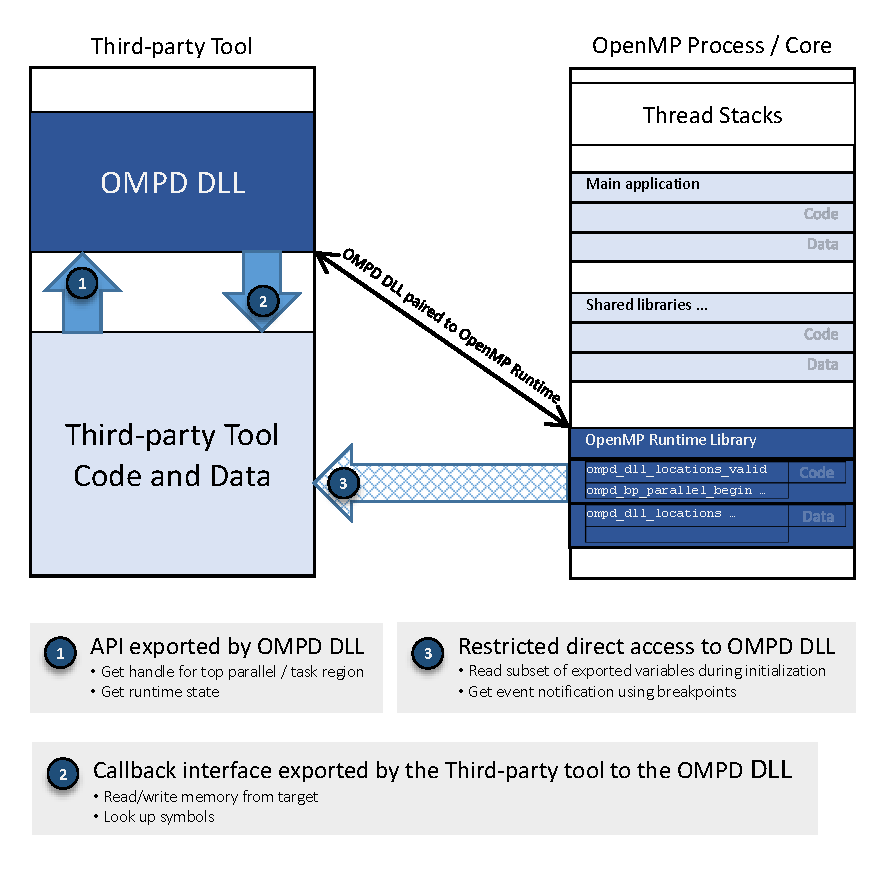
\includegraphics[width=5.0in,natwidth=424.8,natheight=417.6]{figures/ompd-structural-overview.pdf}
%  \caption{OMPD: Structural overview}
%\label{fig:ompd:structural-overview}
%\end{figure}


The diagram shown in  \specref{chap:ompd_diagram} shows how the different
components fits together.
The third-party tool loads the OMPD library that matches the OpenMP runtime
being used by the OpenMP program.
The library exports the API defined later in this document,
which the tool uses to get OpenMP information about the OpenMP program.
The OMPD library will need to look up the symbols,
or read data out of the program.
It does not do this directly, but instead asks the tool to perform
these operations for it using a callback interface exported by the tool.

This architectural layout insulates the tool from the details
of the internal structure of the OpenMP runtime.
Similarly, the OMPD library does not need to be concerned about
how to access the OpenMP program.
Decoupling the library and tool in this way allows for
great flexibility in how the OpenMP program and tool are deployed,
so that, for example, there is no requirement that tool
and OpenMP program execute on the same machine.
Generally the tool does not interact directly with the OpenMP
runtime in the OpenMP program, and instead uses the OMPD library
for this purpose.
However, there are a few instances where the tool does need
to access the OpenMP runtime directly.
These cases fall into two broad categories.
The first is during initialization, where the tool needs
to be able to look up symbols and read variables in OpenMP runtime
in order to identify the OMPD library it should use.
This is discussed in Sections~\ref{subsubsec:ompd_dll_locations}
and~\ref{subsubsec:ompd_dll_locations_valid}.

The second category relates to arranging for the tool to be notified
when certain events occur during the execution of the OpenMP program.
The model used for this purpose is that the OpenMP implementation
is required to define certain symbols in the runtime code.
This is discussed in Section~\ref{subsec:runtime-entry-points-for-ompd}.
Each of these symbols corresponds to an event type.
The runtime must ensure that control passes through the appropriate
named location when events occur.
If the tool wants to get notification of an event, it can plant
a breakpoint at the matching location.

The code locations can, but do not need to, be functions.
They can, for example, simply be labels.
However, the names must have external \texttt{C} linkage.

